\documentclass{article}
\usepackage[margin=1.5cm,bottom=2cm]{geometry}
\usepackage{fancyhdr}
\usepackage{graphicx}
\pagestyle{fancy}
\usepackage{enumitem,amssymb,amsmath}
\newlist{todolist}{itemize}{2}
\setlist[todolist]{label=$\square$}

\begin{document}
\fancyhead[L]{ 
\includegraphics[width=2cm]{au_logo.png} }
\fancyhead[R]{PHYS 2250: General Physics II}
\fancyfoot[C]{\thepage}
\vspace*{0cm}
\begin{center}
	{\LARGE \textbf{Quiz 5}}
	%\vspace{0.25cm}
	%{\Large Due: Friday, September 11}
\end{center}

\begin{enumerate}
	\item In the diagram below, a current $I$ is flowing through a wire of length $d$ along the $y$-axis. The $z$-axis points out of the page. For the following questions, you may leave your answer in the form of an integral, but make sure to evaluate any cross products that arise.
	\begin{figure}[ht!]
		\centering
		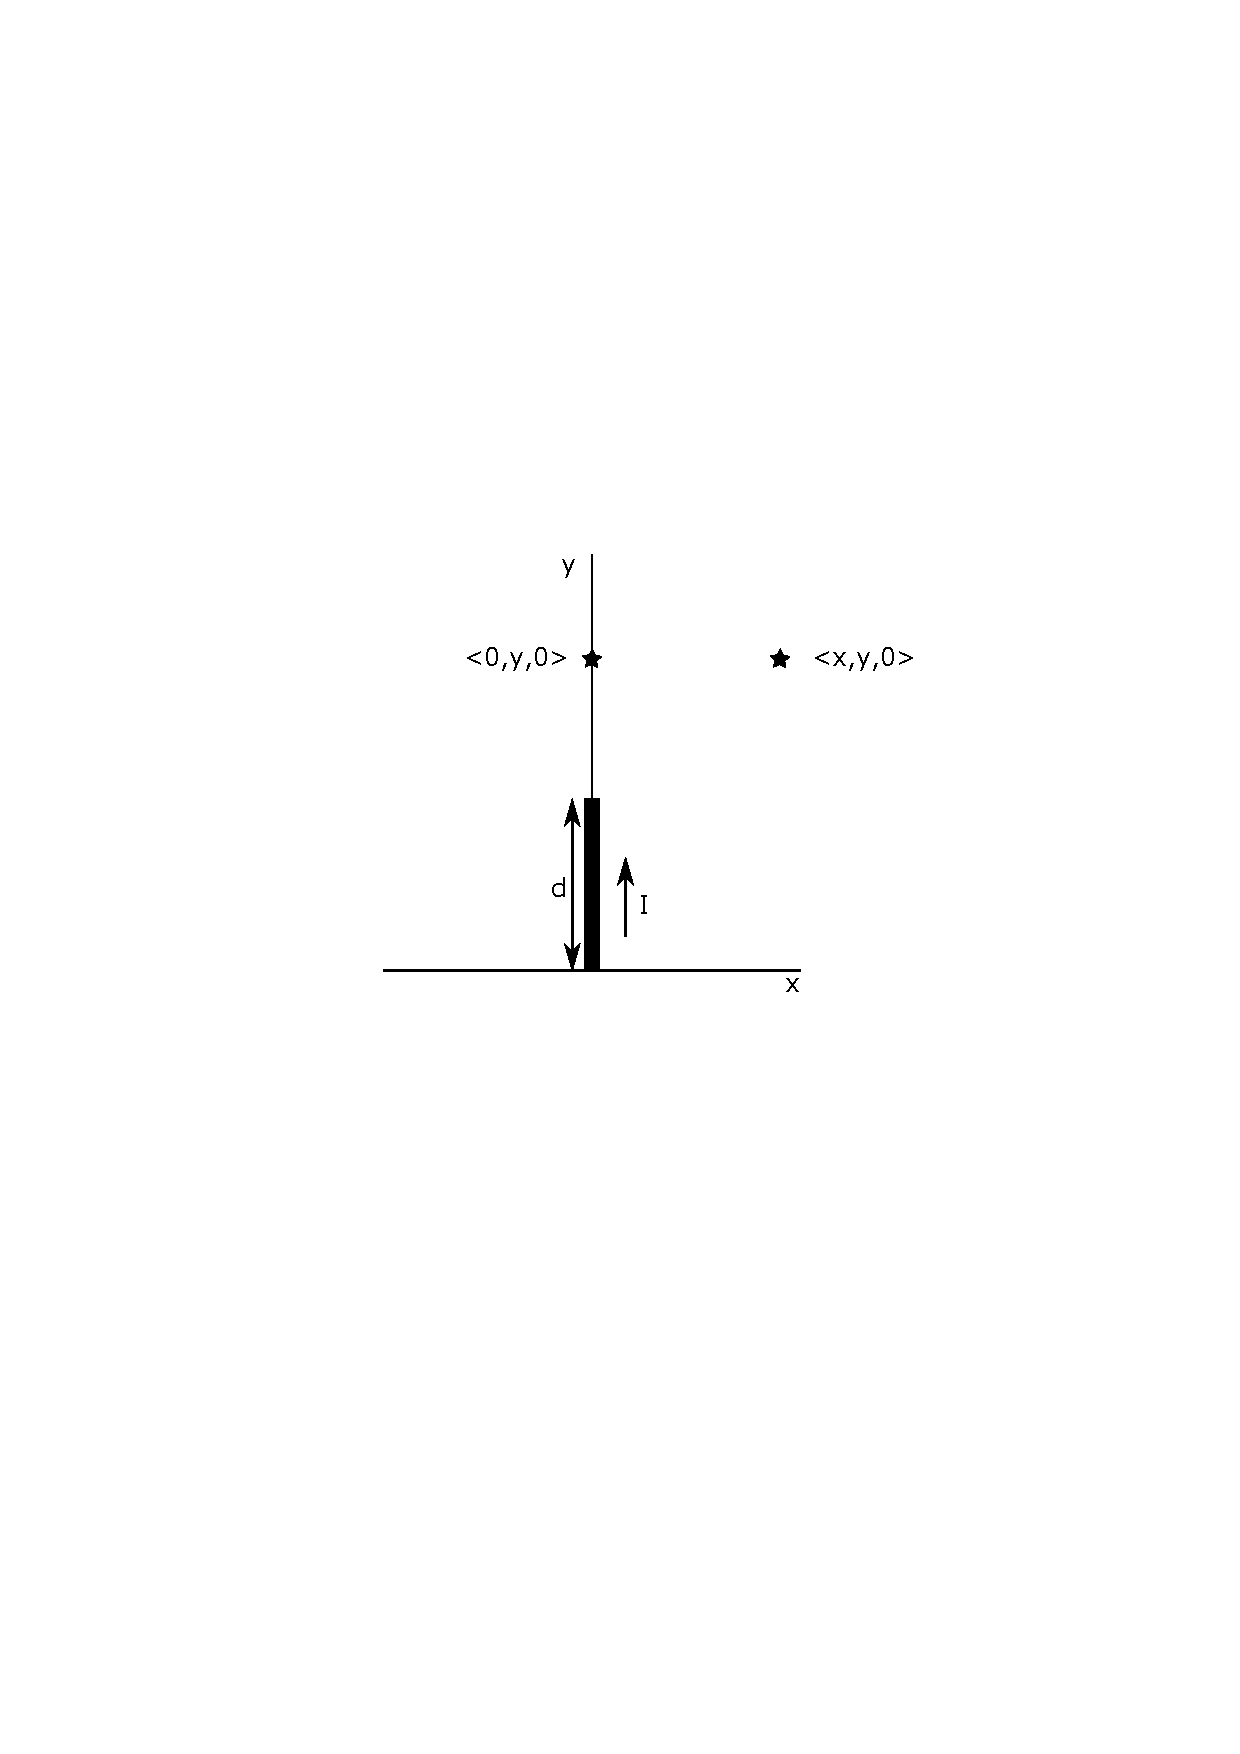
\includegraphics[width=7cm]{current_wire}
	\end{figure}
	\begin{enumerate}
		\item What is the magnetic field vector at a point $<0,y,0>$ along the $y$-axis?
		\vspace{5cm}
		\item What is the magnetic field vector at a point $<x,y,0>$?
	\end{enumerate}
\end{enumerate}

\end{document}